\chapter{Projektowanie i implementacja}
\label{cha:implementacja}

Nakreślony problem -- rozproszonego systemu, który dzięki propagacji danych między użytkownikami obniży obciążenie serwerów sieci Web -- stawia wiele wyzwań projektowych i architektonicznych.

\section{Wymagania funkcjonalne}
\label{sec:funkcjonalnosc}

System dHTTP, z punktu widzenia użytkownika, ma spełniać jedną funkcjonalność: utrzymać lub poprawić płynność dostępu do interesujących go witryn internetowych, nie wpływając na ich treść i nie naruszając prywatności.

Projekt udostępnia interfejs zapewniający dostęp do statystyk, a także preferencji użytkownika. Udostępnione preferencje dotyczą: stopnia działania aplikacji w tle, trybów propagacji i przechowywania danych.
% To może powinno być gdzieś indziej
\begin{figure}[h]
	\centering
    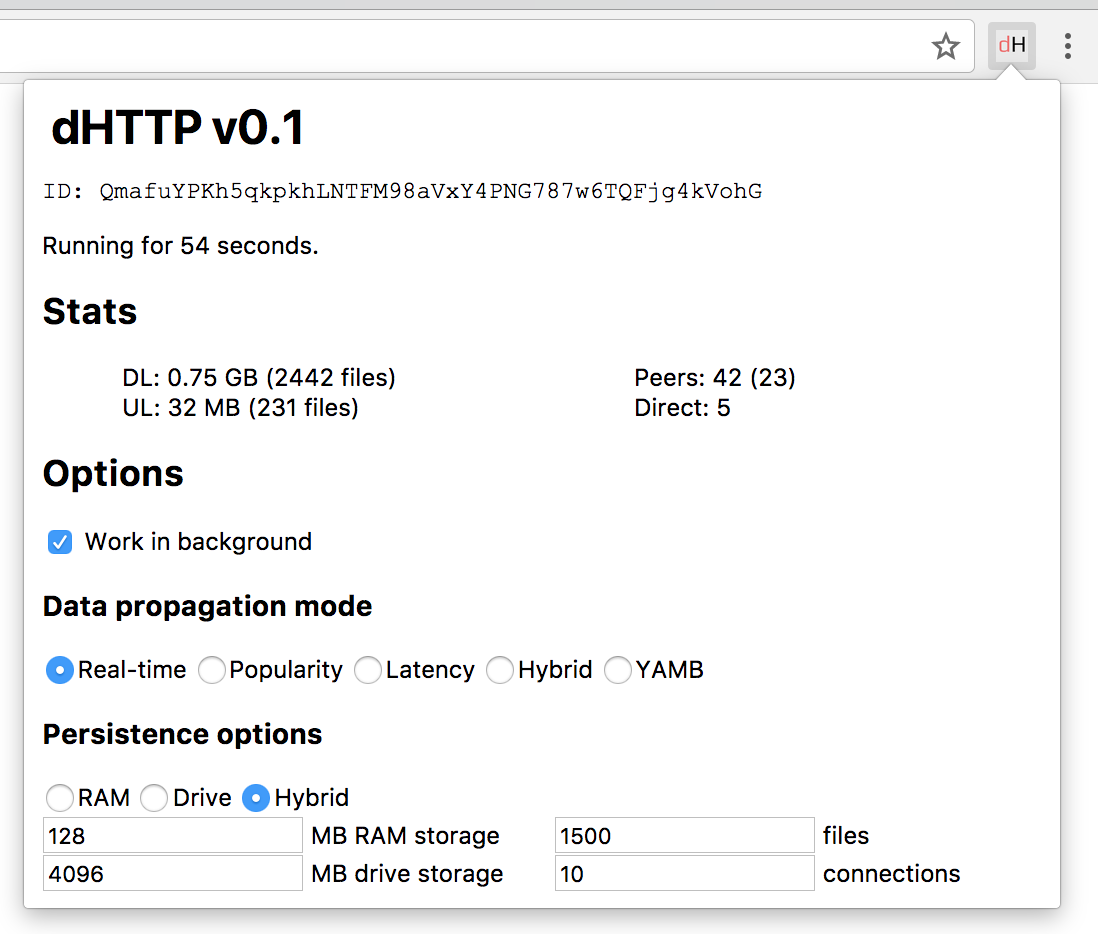
\includegraphics[scale=0.5]{dhttp-initial-interface.png}
	
	\caption{\label{fig:initialInterface} Wstępna implementacja interfejsu operacji dla systemu dHTTP: pop-up dostarczany przez wtyczkę do przeglądarki Google Chrome pozwala na obserwację statystyk i zmianę preferencji.}
\end{figure}

% TODO - gdzieś w pracy podkreśl, jak bardzo istotna jest prosta i automatyczna klastryzacja
Wymogiem dla projektu, koniecznym z racji potrzeby prostej automatyzacji rozrostu sieci, jest tryb niezależny aplikacji -- {\em headless mode} -- pozwalający na wystartowanie niezależnego węzła jednym poleceniem. Niezbędnym jest, aby węzeł tego typu udostępniał statystyki użycia i wstępną konfigurację przy użyciu poleceń interfejsu konsolowego, pozwalając jednak na funkcjonalne uruchomienie z domyślną konfiguracją.


\section{Definicje, architektura i technologie}
\label{sec:zalozeniaProjektu}

W celu uniknięcia niejednoznaczności w dalszym toku pracy, zdefiniowane zostaną następujące pojęcia:

\begin{itemize}
    \item \textbf{węzeł} -- pojedynczy, autonomiczny element systemu, który wykorzystuje komunikację sieciową w celu rozgłaszania i pobierania danych.
    \item \textbf{klaster}
    \item The third etc \ldots
  \end{itemize}

\subsection{Wykorzystane technologie i narzędzia}
\label{sec:techNTools}
\texttt{libp2p} stanowi względnie wysokopoziomową kanwę dla projektu dHTTP.

\subsection{Problemy warstwy sieciowej}
\label{sec:networkIssues}

\subsection{Decentralizacja czy rozproszenie?}
\label{sec:decentralizacjaCzyRozproszenie}

\subsection{Bezpieczeństwo}
\label{sec:security}

\subsubsection{Czy autentykacja to nasza brożka?}
\subsubsection{Gdzie leżą granice zdrowych heurystyk?}

\subsection{Propagacja i przechowywanie danych}
\label{sec:dataPropagation}

% Z tego poniżej może powstać osobny rozdział, gdzie to co powyżej stanowiłoby bardziej rozważania na temat właściwego podejścia do realizacji projektu, a to poniżej -- faktyczny opis implementacji systemu, podzielony bardziej granularnie dla każdego z elemenetów

\section{Aplikacje}

\subsection{Węzeł}
\subsection{Klient}

